\section{Neural Network Approach}
\label{neural_network}
Our approach for building our convolutional neural network is to start with a baseline network to see what the results we can get from the start. From then on we can branch out and tweak with different network structures and hyper parameters to see how far we can fine tune and improve it to get better results.
We will base our approach by using the pre-trained Inception V3 network as the base for what we will build upon in a technique called transfer learning. This allows us to take advantage of an already fully trained powerful classification model that we can use to retrain for a new set of classes. By doing this, we can get pretty decent results out of the box this way which will cut down on the amount of work needed to train a completely new network from scratch as there isn’t enough time or data available. We will be using this pre-trained network in order to extract features for the 3 new Rock, Paper, Scissors classes which will help in classifying them. We will also be fine tuning the weights of the pre-trained network by retraining some of the later layers in the network in order to conform to our dataset as these later layers may contain weights specific to the ImageNet classes.

\begin{figure}[h]
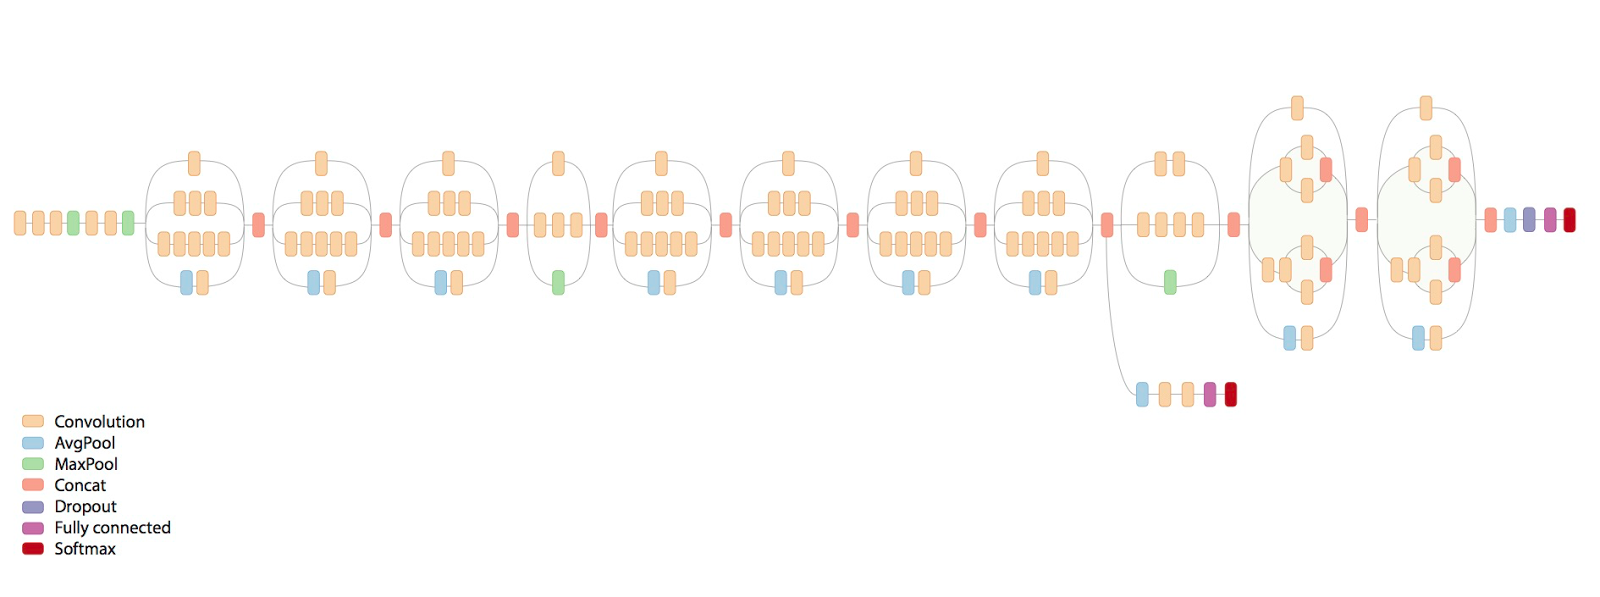
\includegraphics[scale=0.3]{nn_pic.png}
\centering
\caption{The original inception V3 network structure}
\end{figure}

Each network we produce will be trained for 300 epochs using all 215 training and 196 validation images per epoch. Each network can then be benchmarked to see if improvements were made in terms of accuracy and validation accuracy and we can choose the one with the best results are our network of choice.
\subsection{Experiments}

For our neural network, we will experiment with differing network structures and hyperparameters while iterating to see which one performs the best.
\subsubsection{Baseline}
This network was our starting point and is quite simple. It takes the Inception V3 model and replaces the last dense layer with 3 more layers, a 32 node fully connected layer, a dropout layer and finally the output layer (with 3 output nodes for our classes). The output layer uses the softmax activation whereas the fully connected layer uses ReLU. This network was trained with the loss function set to categorical cross entropy and the optimizer set to stochastic gradient descent (with a learning rate of 0.01).

Results: Accuracy – 98\%, Validation Accuracy – 78\%

With this baseline network, it seems that our validation accuracy is not that great. The way to go and improve that is to use regularization to reduce overfitting. The simple way to do this is with dropout layers which sets a fraction of the input units to 0 at each update during training. Our baseline network already includes a single dropout layer before the classification layer, but it did not look like it was enough.
\subsubsection{Network 1}

Network1 consisted of replacing the top classification layer of Inception V3 and adding a GlobalAveragePooling2D layer, 32 node fully connected layer, a dropout layer, and finally the output layer. This time, the dropout was increased to 0.8 to see if that will improve our validation accuracy. For training, the layers that we added were trained first using rmsprop as the optimizer while everything else was frozen, then the last two blocks of Inception V3 were unfrozen and the network was trained again. This time for stochastic gradient descent, we went with a learning rate of 0.0001 and momentum of 0.9.

Results: Accuracy – 92\%, Validation Accuracy – 78\%

This time, the accuracy went down but the validation accuracy didn’t improve.
\subsubsection{Network 2}

For network2, we simply tried training all the layers from network1 in one go.

Results: Accuracy – 92\%, Validation Accuracy – 73\%

This made things worse as the accuracy was the same but the validation accuracy dropped down to around 73%.
\subsubsection{Network 3}

For network3, we decided to add another dropout layer onto network2 after the GlobalAveragePooling2D layer with it set at 0.5, just to see if it helps anymore with overfitting. 

Results: Accuracy – 99\%, Validation Accuracy – 78\%

The results were that the accuracy surprisingly went up for both, this seemed more promising.
\subsubsection{Network 4}

We saw from network3 that adding another dropout layer made our validation accuracy better, so why not do it again. For network4 we added another dropout layer to just before the GlobalAveragePooling2D layer, also with it set to 0.5. 

Results: Accuracy – 99\%, Validation Accuracy – 80\%

This time, the accuracy was still at 99\% but the validation accuracy improved again to around 80\%, so things are improving slowly.
\subsubsection{Network 5}

For network5, we took network4 but trained it in two steps like in network 1 – the layers that we added were trained first using rmsprop as the optimizer while everything else was frozen, then the last two blocks of Inception V3 were unfrozen and the network trained again. 

Results: Accuracy – 99\%, Validation Accuracy – 77\%

The accuracy remained at 99\% but validation accuracy dropped to around 77\%, which is not any better.
\subsubsection{Network 6}

From network5, it looked like the validation accuracy was oscillating quite a bit around the 77\% range, so for network6 we set the stochastic gradient descent parameters to have a momentum of 0 and a learning rate of 0.01.

Results: Accuracy – 100\%, Validation Accuracy – 84\%

This proved to be the most promising so far as accuracy went to 100\% and validation accuracy went to 84\%, which is the best so far.
\subsubsection{Network 7}

From what we learned from network6 is that our validation accuracy varied a lot depending on our stochastic gradient descent parameters. It seems like we may be stuck at some local minima in our loss function. For network7 we removed the dropout layer just before the GlobalAveragePooling2D layer. This time we tweaked with the hyperparameters even more, setting the learning rate to 0.01, learning rate decay to 1e-6 and momentum to 0.9

Results: Accuracy – 100\%, Validation Accuracy – 90\%

This proved to give the best results that we could get with accuracy of 100\% and validation accuracy of 90\%, which is a huge improvement over network6.
\subsubsection{Network 8}

This network just added back the dropout layer that was removed in network7.

Results: Accuracy – 100\%, Validation Accuracy – 85\%

The results were similar, but the validation accuracy oscillated a lot between 82-90\%.
\subsection{Observations}
During training, we found out that 300 epochs was usually where the training and validation accuracy would plateau. Beyond that point, the results did not improve significantly. This is probably due to the fact that dataset was simply too small. If we had a lot more data, then our results may have improved some more.
We also noticed that when our network classified an image wrong, it was usually totally off. For example, the classification score for an image would be 0.99 for Paper when it was actually Scissors. This was the case for a lot of the images that it got wrong. It would be quite certain that an image is of one class, but be off completely. This is most likely due to overfitting as our dataset did not have enough varying examples.
